\chapter{\ifenglish Background Knowledge and Theory\else ทฤษฎีที่เกี่ยวข้อง\fi}

เนื้อหาในบทนี้อธิบายทฤษฎีและเทคโนโลยีที่เกี่ยวข้องกับโครงงานนี้

\section{Field of View}
Field of View (FOV) คือมุมที่กล้องมองเห็น เมื่อติดตั้งกล้องให้มองลงตั้งฉากกับพื้น ความกว้างของพื้นที่ที่กล้องเห็นบนพื้นคำนวณได้จากมุม FOV และระยะห่างจากกล้องถึงพื้น

\begin{equation}\label{eq:field-of-view-objt}
  L = 2D \tan\left(\frac{\theta}{2}\right)
\end{equation}

โดยที่ L คือความกว้างของพื้นที่ที่มองเห็น D คือระยะจากกล้องถึงพื้นที่ทำงาน และ $θ$ คือมุมมองของกล้องในแนวนอนหรือแนวตั้ง

\begin{figure}[htbp]
  \centering
  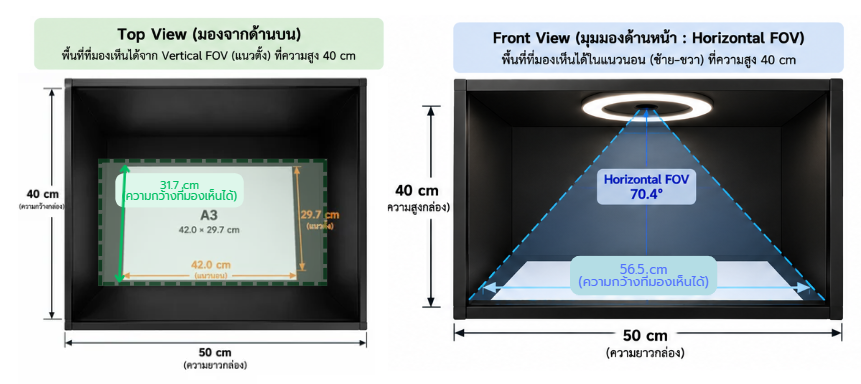
\includegraphics[width=0.95\textwidth]{images/field_of_view.png}
  \caption{Field of View ของกล้อง}
  \label{fig:field-of-view}
\end{figure}

\section{การวัดขนาดวัตถุจากภาพด้วยวัตถุอ้างอิง (Reference Object Calibration)}

กระบวนการปรับเทียบค่ามาตราส่วน (Scale Calibration) หรือการหาความสัมพันธ์ระหว่าง ``หน่วยพิกเซล (pixel)'' ในภาพดิจิทัล กับ ``ขนาดหรือระยะทางจริงในโลกแห่งความจริง (real-world units)'' โดยใช้วัตถุอ้างอิง (Reference Object) ที่ทราบขนาดที่แน่นอนอยู่แล้ววางไว้ในภาพเดียวกัน แล้วคำนวณอัตราส่วนระหว่างหน่วยจริงกับพิกเซล

\begin{equation}\label{eq:reference-object}
  s = \frac{L_{ref}}{N_{ref}} \quad [\text{mm/pixel}], \quad L_{obj} = s \cdot N_{obj}
\end{equation}

โดยที่ $L_{ref}$ คือขนาดจริงของวัตถุอ้างอิง $N_{ref}$ คือขนาดของวัตถุอ้างอิงเป็นพิกเซล และ $N_{obj}$ คือขนาดของสกรูเป็นพิกเซล

\section{การประมวลผลภาพ (Image Processing)}\label{sec:2.3}

การประมวลผลภาพ (Image Processing) คือ กระบวนการนำภาพทางดิจิทัลมาผ่านการประมวลผลด้วยระบบคอมพิวเตอร์และขั้นตอนทางคณิตศาสตร์ เพื่อปรับปรุงคุณภาพของรูปภาพให้มองเห็นรายละเอียดได้ชัดเจนยิ่งขึ้น หรือเพื่อวิเคราะห์และสกัดเอาข้อมูลเฉพาะเจาะจงที่ซ่อนอยู่ในภาพออกมาใช้งานต่อ ในอุตสาหกรรมการผลิต เทคโนโลยีนี้ถูกนำมาประยุกต์ใช้อย่างแพร่หลายสำหรับระบบตรวจสอบคุณภาพอัตโนมัติ (Automated Defect Inspection) การคัดแยกชิ้นงาน และการวัดขนาดวัตถุแบบไม่สัมผัส ซึ่งช่วยลดความผิดพลาดจากมนุษย์ (Human Error) และเพิ่มความรวดเร็วในสายการผลิตได้อย่างแม่นยำ \cite{dia2024,ikki2023}

\section{การตรวจจับขอบด้วย Canny (Canny Edge Detection)}

ขอบ (edge) คือตำแหน่งที่ความเข้มแสงเปลี่ยนแปลงอย่างรวดเร็ว เช่น รอยต่อระหว่างสกรูกับพื้นหลัง Canny Edge Detector ที่เสนอโดย John Canny ในปี 1986 เป็นอัลกอริทึมที่นิยมที่สุด เพราะออกแบบให้ตรวจจับขอบได้ถูกต้อง ตำแหน่งแม่นยำ และได้เส้นขอบบางเพียงหนึ่งพิกเซล \cite{wikipediaCanny2024,canny1986,opencvCanny2024} ประกอบด้วย 5 ขั้นตอน ดังนี้

\subsection{Gaussian Filter}

กรองภาพด้วยฟังก์ชันเกาส์เซียนสองมิติ เพื่อลดสัญญาณรบกวนและป้องกันการตรวจพบขอบเท็จ (false detection) ที่เกิดจาก noise

\begin{equation}\label{eq:gaussian-filter}
  G(x,y) = \frac{1}{2\pi\sigma^2} \exp\left(-\frac{x^2+y^2}{2\sigma^2}\right)
\end{equation}

ค่า $σ$ คือค่าเบี่ยงเบนมาตรฐานที่กำหนดความกว้างของการเบลอ ภาพตัวอย่างในสไลด์แสดงว่า $σ$ = 1 ให้ขอบละเอียดแต่มีขอบจากรายละเอียดเล็กจำนวนมาก ส่วน $σ$ = 2 และ $σ$ = 4 ให้ขอบน้อยลงและเหลือเฉพาะโครงร่างหลัก จึงต้องเลือก $σ$ ให้พอเหมาะกับขนาดของสกรูและสัญญาณรบกวนในภาพ

\subsection{Gradient Calculation}

คำนวณเกรเดียนต์ของความเข้มแสงในแนวนอน (Gx) และแนวตั้ง (Gy) ซึ่งนิยมใช้เคอร์เนล Sobel ขนาด 3 × 3 เพื่อหาขนาดและทิศทางของขอบ \cite{firstprinciples2021canny}

\begin{equation}\label{eq:gradient-calculation}
  |G| = \sqrt{G_x^2 + G_y^2}, \quad \theta = \arctan\left(\frac{G_y}{G_x}\right)
\end{equation}

ขนาด |G| บอกความแรงของขอบ ส่วนมุม $θ$ บอกทิศทางที่ตั้งฉากกับเส้นขอบ

\subsection{Non-Maximum Suppression}

หลังจากได้ค่าขนาด (Gradient Magnitude) และทิศทาง (Gradient Direction) ของเกรเดียนต์แล้ว จะทำการสแกนภาพทั้งหมดเพื่อลบพิกเซลที่ไม่ต้องการ ซึ่งอาจไม่ใช่ส่วนหนึ่งของขอบภาพ (Edge) โดยวิธีนี้จะตรวจสอบพิกเซลทุกพิกเซลว่า เป็นค่าจุดสูงสุดเฉพาะที่ (Local Maximum) ในบริเวณใกล้เคียงตามทิศทางของเกรเดียนต์หรือไม่ หากพิกเซลนั้นไม่ใช่ค่าจุดสูงสุดเฉพาะที่ ก็จะถูกลบออก

\begin{figure}[H]
  \centering
  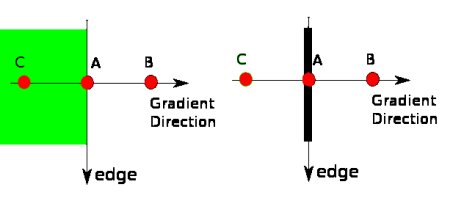
\includegraphics[width=0.7\textwidth]{images/non-maximum-suppression.png}
  \caption{Non-Maximum Suppression}
  \label{fig:non-maximum-suppression}
\end{figure}

จุด A อยู่บนขอบภาพ (Edge) ซึ่งมีทิศทางเป็นแนวตั้ง โดยทิศทางของเกรเดียนต์ (Gradient Direction) จะตั้งฉากกับขอบภาพ

จุด B และ C อยู่ในทิศทางเดียวกับเกรเดียนต์ ดังนั้นจึงนำค่าของจุด A ไปเปรียบเทียบกับจุด B และ C เพื่อตรวจสอบว่าจุด A เป็นค่าจุดสูงสุดเฉพาะที่ (Local Maximum) หรือไม่
\begin{itemize}                
  \item ถ้าใช่: จุด A จะถูกเก็บไว้เพื่อเข้าสู่ขั้นตอนถัดไป
  \item ถ้าไม่ใช่: จุด A จะถูกตัดออก โดยกำหนดค่าเป็นศูนย์ (0)
\end{itemize}

\subsection{Double Thresholding}

กำหนดเกณฑ์ 2 ค่า คือ Th (สูง) และ Tl (ต่ำ) เพื่อแบ่งพิกเซลขอบเป็น 3 กลุ่ม \cite{opencvCanny2024}

\begin{table}[htbp]
  \centering
  \begin{tabular}{|l|l|l|}
    \hline
    \textbf{กลุ่ม} & \textbf{เงื่อนไข}                 & \textbf{ความหมาย}      \\ \hline
    Strong edge  & $|G| \ge \text{Th}$             & เชื่อว่าเป็นขอบจริงและเก็บไว้ \\ \hline
    Weak edge    & $\text{Tl} \le |G| < \text{Th}$ & ยังไม่แน่นอน รอตรวจสอบ    \\ \hline
    Non-edge     & $|G| < \text{Tl}$               & ไม่ใช่ขอบ ตัดทิ้ง           \\ \hline
  \end{tabular}
  \caption{แสดงการแบ่งกลุ่มของขอบภาพ (Edge Groups)}
  \label{tab:edge-groups}
\end{table}

\subsection{Edge Tracking by Hysteresis}

ตรวจสอบ weak edge ว่าเชื่อมต่อกับ strong edge หรือไม่ หากเชื่อมต่อจะเก็บไว้เป็นขอบ หากอยู่โดดเดี่ยวจะถูกลบออก ช่วยให้ได้ขอบที่ต่อเนื่องและแม่นยำ โดยไม่เก็บขอบจาก noise

\begin{figure}[H]
  \centering
  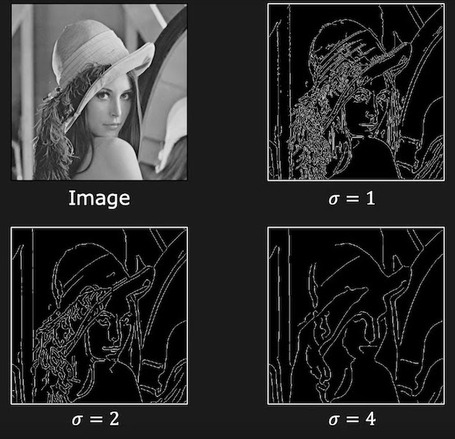
\includegraphics[width=0.7\textwidth]{images/canny-edge-detection-method.jpg}
  \caption{เปรียบเทียบผลลัพธ์การตรวจจับขอบตามค่า $\sigma$ ที่แตกต่างกัน}
  \label{fig:canny-sigma-comparison}
\end{figure}

\section{Segmentation และ Edge Following}

Segmentation คือการแบ่งภาพเพื่อแยกวัตถุที่สนใจออกจากพื้นหลัง ในโครงงานนี้คือการแยกสกรูแต่ละตัวออกจากพื้นหลังสีขาวของพื้นที่งาน โดยใช้ขอบที่ได้จาก Canny

Edge Following คือการไล่ตามพิกเซลขอบที่เชื่อมต่อกันจนครบรอบวัตถุ เพื่อได้เส้นรอบรูป (Contour) หนึ่งเส้นต่อวัตถุหนึ่งชิ้น ผลลัพธ์นี้นำไปใช้สามอย่างคือ นับจำนวนสกรู (หนึ่ง Contour เท่ากับหนึ่งตัว) วาดกรอบรอบสกรูเพื่อแสดงผล Visual Detection และใช้เป็นฐานวัดขนาดในหัวข้อนี้

\subsection{ปัญหาวัตถุวางซ้อนทับ (Overlap)}

เมื่อสกรูวางชิดกันจนเส้นขอบเชื่อมติดกัน (Contour เชื่อมติดกัน) ระบบจะเห็นเป็นวัตถุชิ้นเดียว ทำให้นับจำนวนและวัดขนาดผิด โครงงานนี้จึงแก้ที่ต้นเหตุด้วยข้อแนะนำการจัดวาง คือวางสกรูแยกกันชัดเจน แสงสว่างสม่ำเสมอ เงาน้อย และพื้นหลังสีขาวที่มีแสงสะท้อนน้อย ตามรูปภาพ Placement Guidelines

\section{การจำแนกประเภท (Classification)}

การจำแนกประเภทภาพ (Image Classification) หรือการจัดกลุ่มภาพ คือกระบวนการทางคอมพิวเตอร์วิทัศน์ (Computer Vision) ที่ใช้ในการระบุและจัดหมวดหมู่ของวัตถุที่ปรากฏอยู่ในภาพ โดยระบบจะวิเคราะห์คุณลักษณะและข้อมูลของภาพ จากนั้นจึงทำการติดป้ายกำกับ (Label) เพื่อบอกว่าภาพหรือวัตถุนั้นคือสิ่งใดตามหมวดหมู่ที่ได้กำหนดไว้ล่วงหน้า